%%%%%%%%%%%%%%%%%%%%%%%%%%%%%%%%%%%%%%%%%
% Beamer Presentation
% LaTeX Template
% Version 1.0 (10/11/12)
%
% This template has been downloaded from:
% http://www.LaTeXTemplates.com
%
% License:
% CC BY-NC-SA 3.0 (http://creativecommons.org/licenses/by-nc-sa/3.0/)
%
%%%%%%%%%%%%%%%%%%%%%%%%%%%%%%%%%%%%%%%%%

%----------------------------------------------------------------------------------------
%	PACKAGES AND THEMES
%----------------------------------------------------------------------------------------

\documentclass{beamer}

\mode<presentation> {

% The Beamer class comes with a number of default slide themes
% which change the colors and layouts of slides. Below this is a list
% of all the themes, uncomment each in turn to see what they look like.

%\usetheme{default}
%\usetheme{AnnArbor}
%\usetheme{Antibes}
%\usetheme{Bergen}
%\usetheme{Berkeley}
%\usetheme{Berlin}
%\usetheme{Boadilla}
%\usetheme{CambridgeUS}
%\usetheme{Copenhagen}
%\usetheme{Darmstadt}
%\usetheme{Dresden}
%\usetheme{Frankfurt}
%\usetheme{Goettingen}
%\usetheme{Hannover}
%\usetheme{Ilmenau}
%\usetheme{JuanLesPins}
%\usetheme{Luebeck}
%\usetheme{Madrid}
%\usetheme{Malmoe}
%\usetheme{Marburg}
%\usetheme{Montpellier}
%\usetheme{PaloAlto}
%\usetheme{Pittsburgh}
\usetheme{Rochester}
%\usetheme{Singapore}
%\usetheme{Szeged}
%\usetheme{Warsaw}

% As well as themes, the Beamer class has a number of color themes
% for any slide theme. Uncomment each of these in turn to see how it
% changes the colors of your current slide theme.

%\usecolortheme{albatross}
%\usecolortheme{beaver}
%\usecolortheme{beetle}
%\usecolortheme{crane}
%\usecolortheme{dolphin}
%\usecolortheme{dove}
%\usecolortheme{fly}
%\usecolortheme{lily}
%\usecolortheme{orchid}
%\usecolortheme{rose}
%\usecolortheme{seagull}
%\usecolortheme{seahorse}
%\usecolortheme{whale}
%\usecolortheme{wolverine}

%\setbeamertemplate{footline} % To remove the footer line in all slides uncomment this line
%\setbeamertemplate{footline}[page number] % To replace the footer line in all slides with a simple slide count uncomment this line

\setbeamertemplate{navigation symbols}{} % To remove the navigation symbols from the bottom of all slides uncomment this line

\definecolor{OUGold}{RGB}{181,154,57}
\setbeamercolor{structure}{fg=OUGold}
\setbeamercolor{block title example}{bg=OUGold}
\setbeamercolor{section in toc}{fg=black}

% position the logo
\addtobeamertemplate{frametitle}{}{%
	\begin{textblock*}{\paperwidth}(290pt,-38pt)
		
\includegraphics[height=1cm,keepaspectratio]{sail}
	\end{textblock*}}
}

\usepackage{textpos} % package for the positioning
\usepackage{graphicx} % Allows including images
\usepackage{booktabs} % Allows the use of \toprule, \midrule and \bottomrule in tables
\usepackage{pdfpages} % Allows including PDFs (in separate frame)

%----------------------------------------------------------------------------------------
%	TITLE PAGE
%----------------------------------------------------------------------------------------

\title[Bank Marketing Project]{Text Mining Project: Presentation 1} % The short title appears at the bottom of every slide, the full title is only on the title page

\author{Evan Bradley} % Your name
\institute[OU] % Your institution as it will appear on the bottom of every slide, may be shorthand to save space
{
Oakland University \\ % Your institution for the title page
\medskip
\textit{edbradley@oakland.edu} % Your email address
}
\date{November 2016} % Date, can be changed to a custom date

\begin{document}

\begin{frame}
	\frametitle{\space}
	\titlepage % Print the title page as the first slide
\end{frame}

\begin{frame}
\frametitle{Overview} % Table of contents slide, comment this block out to remove it
\tableofcontents % Throughout your presentation, if you choose to use \section{} and \subsection{} commands, these will automatically be printed on this slide as an overview of your presentation
\end{frame}

%----------------------------------------------------------------------------------------
%	PRESENTATION SLIDES
%----------------------------------------------------------------------------------------

%------------------------------------------------
\section{Sources of Data} % Sections can be created in order to organize your presentation into discrete blocks, all sections and subsections are automatically printed in the table of contents as an overview of the talk
%------------------------------------------------

%\subsection{Test} % A subsection can be created just before a set of slides with a common theme to further break down your presentation into chunks

%------------------------------------------------

% Collected data stats
% Collection and preprocessing with Node.js
% Analysis using R
% Already produced results
% Goals for analysis

\begin{frame}
	\frametitle{Twitter Queries}
	\begin{itemize}
		\item \#Election2016 
		\newline
		\item \#NotMyPresident
		\newline
		\item \#ElectionNight
		\newline
		\item \#ElectionFinalThoughts
		\newline
		\item ``clinton''
		\newline
		\item ``trump'' 
		\newline
	\end{itemize}
\end{frame}

\begin{frame}
	\frametitle{Collected Data}
	\begin{itemize}
    \item Around 1,000,000 tweets 
    \newline
    \item Drawing from hashtags on previous slide.
    \newline
    \item Collected from Twitter's stream API
    \newline
    \item Roughly 750,000 tweets per 24 hours.
    \newline
	\end{itemize}
\end{frame}

\begin{frame}
	\frametitle{Collection Process}
	\begin{itemize}
    \item Using Node.js with the Twit module.
    \newline
    \item Responses are written to an output JSON file.
    \newline
    \item Node.js also used to trim data down and convert to CSV.
    \newline
    \item Database should probably be used for data collection (MongoDB).
    \newline
    \item Further pre-processing may be necessary before exporting to CSV.
    \newline
	\end{itemize}
\end{frame}

% ------------------------------------------------
\section{Analysis with R} % Sections can be created in order to organize your presentation into discrete blocks, all sections and subsections are automatically printed in the table of contents as an overview of the talk
%------------------------------------------------

\begin{frame}
	\frametitle{R Packages}
	\begin{itemize}
    \item tm: provides text mining processes (cleaning, TDM, DTM).
    \newline
    \item SnowballC: word-stemming using Porter's algorithm.
    \newline
    \item ggplot2: Plotting library.
    \newline
    \item wordcloud: Produces a wordcloud visualization of word frequency.
    \newline
    \item sentiment: Performs rudimentary sentiment analysis on data.
    \newline
	\end{itemize}
\end{frame}

\begin{frame}
  \frametitle{Word Frequencies}
  \center
  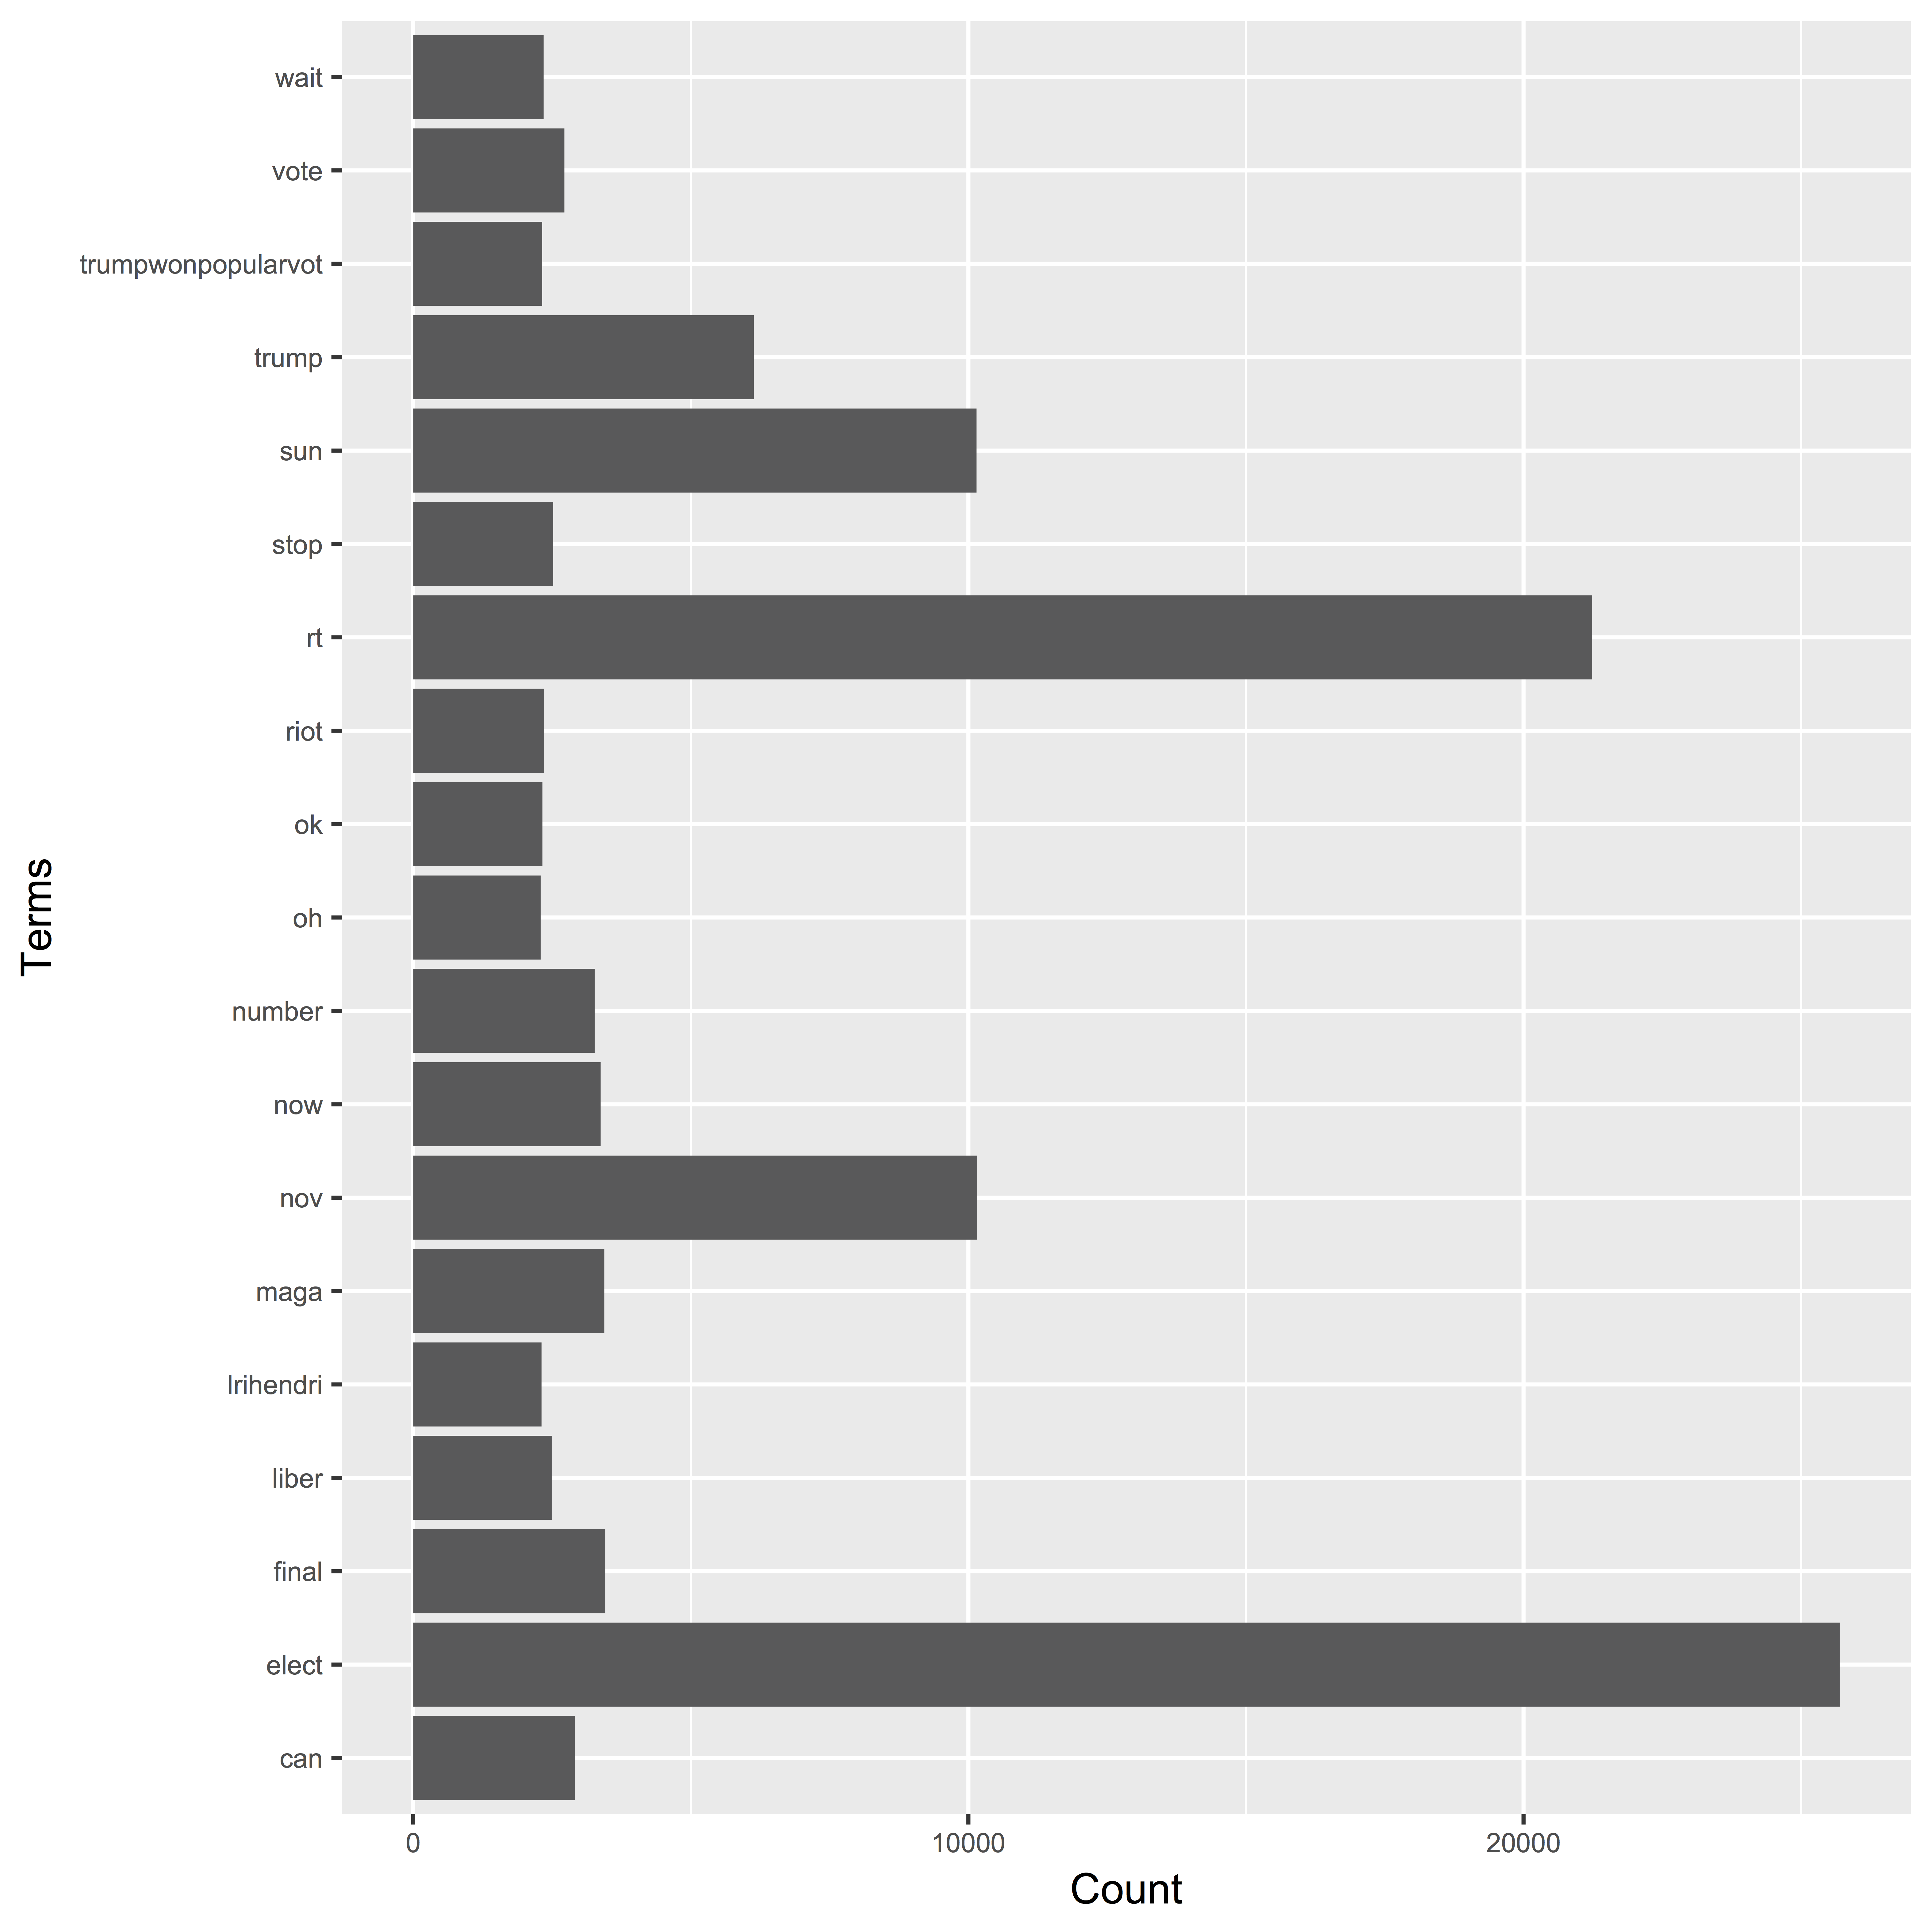
\includegraphics[height = 0.9\textheight]{freqplot}
\end{frame}

\begin{frame}
  \frametitle{Wordcloud}
  \center
  
\includegraphics[height = \textheight]{wordcloud}
\end{frame}

\begin{frame}[fragile]
  \frametitle{Word Associations}
  \begin{verbatim}
> findAssocs(tdm, "trump", 0.2)
$trump
  election  clinton  popularvote  donald electoralcolleg
      0.31     0.28         0.26    0.25            0.22
       won
      0.22

> findAssocs(tdm, "clinton", 0.2)
$clinton
    popularvote electoralcolleg  number  trump  final
           0.55            0.47    0.43   0.28   0.20
  \end{verbatim}
\end{frame}

\begin{frame}[fragile]
  \frametitle{Sentiment Analysis}
  \begin{verbatim}
> sentiments <- sentiment(tweets$text)
> table(sentiments$polarity)

negative  neutral positive
       2      423       63
  \end{verbatim}
\end{frame}

%------------------------------------------------
\section{Tasks for Text Mining}
%------------------------------------------------

\begin{frame}
	\frametitle{Tasks for Text Mining}
	\begin{itemize}
    \item Observe hashtag and topic trends over time.
    \newline
    \item Look at sentiment analysis of election over time.
    \newline
    \item Observe association of terms between Clinton, Trump, and possibly
      other figures.
    \newline
    \item Observe association between hashtags over time.
    \newline
    \item Emoji Analysis
    \newline
	\end{itemize}
\end{frame}

%----------------------------------------------------------------------------------------

\end{document} 
